% =====================================================================
%  Figure captions for: Meibutsu, an inverse instrument for chemical
%  structure
%
%  Every quantity quoted below is read from
%  results/exp_generator.json or recomputed from the instrument.
% =====================================================================

\begin{figure*}[!htbp]
    \centering
    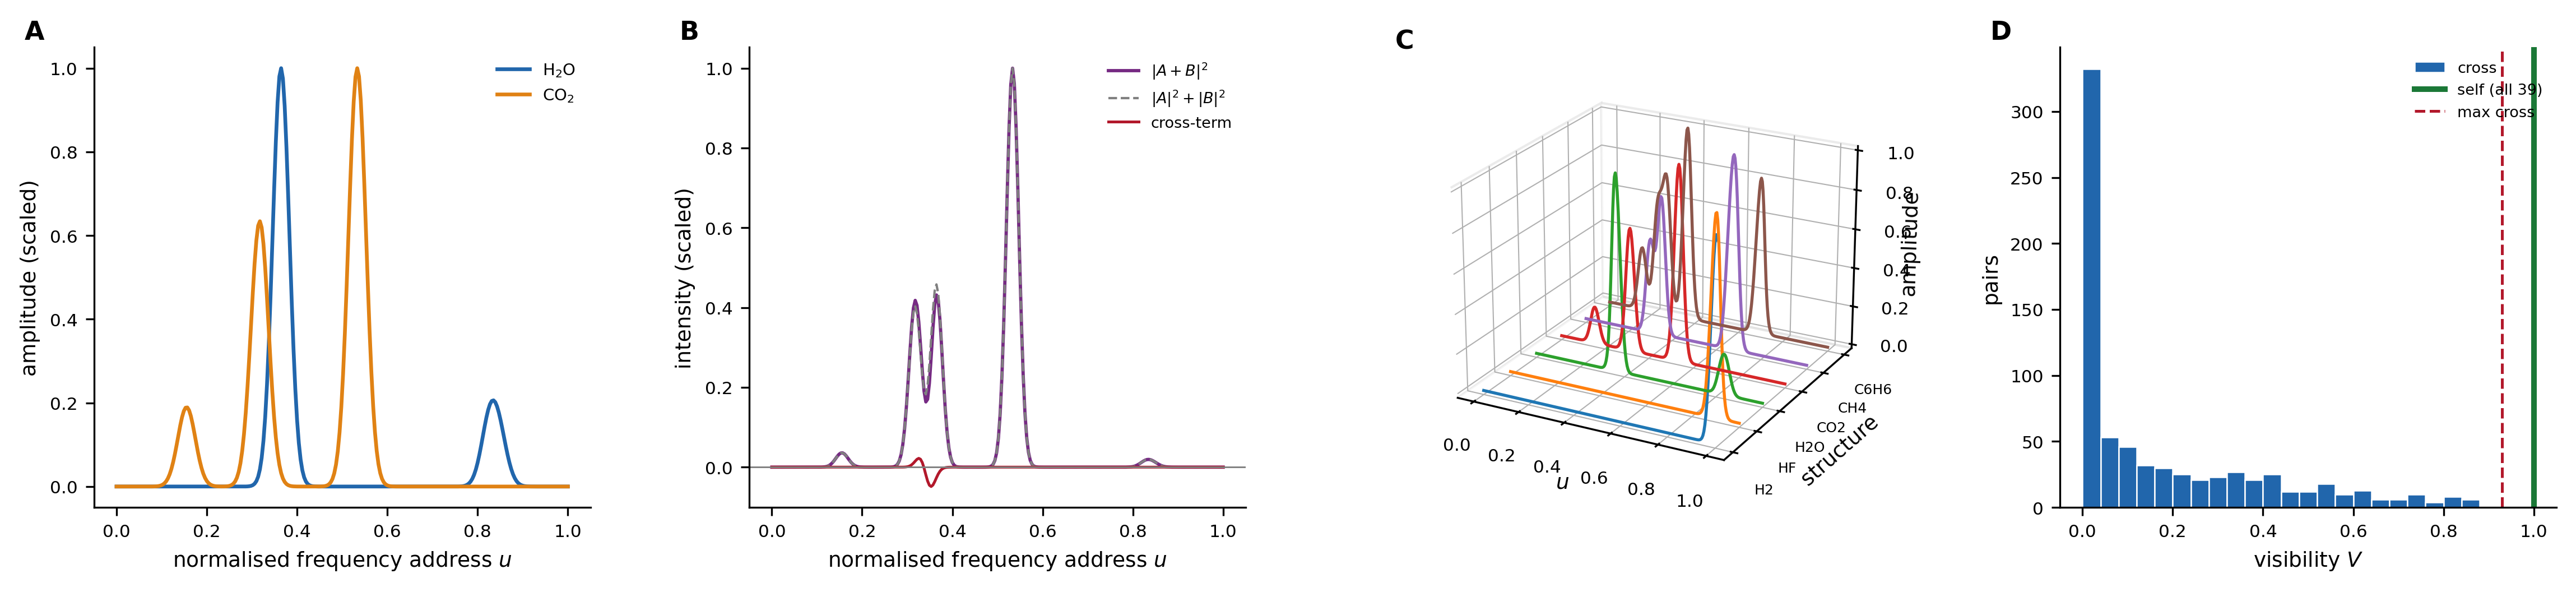
\includegraphics[width=\textwidth]{figures/panel_01_field.png}
    \caption{\textbf{Two structures are compared by adding their fields;
    everything relational lives in the cross-term, and it is small and
    local.}
    All fields are evaluated on a $G=256$ grid with reference frequency
    $\wref=4401$~cm$^{-1}$ (\Cref{def:field}); no quantity here is fitted.
    (\textbf{A})~Amplitude of the observation field for
    H$_2$O and CO$_2$, each scaled to its own maximum. One lobe appears
    per vibrational mode at that mode's normalised frequency address,
    with width set by the first coordinate and envelope by the second.
    The two structures overlap only near $u\approx0.35$, which is where
    panel~(\textbf{B}) finds the entire relational signal.
    (\textbf{B})~The superposition $|A+B|^2$ (purple) against the sum of
    the individual intensities $|A|^2+|B|^2$ (grey dashed) and the
    cross-term $2\operatorname{Re}(\bar A B)$ (red), all scaled by the
    same constant. The purple and grey curves are nearly coincident
    because the cross-term is small: these two structures share little.
    Where the modes do not overlap the cross-term is identically zero ---
    unrelated parts contribute \emph{nothing} rather than contributing a
    small similarity, which is \Cref{prop:cross} in visible form.
    (\textbf{C})~Amplitude fields for six structures spanning the
    reference set, from H$_2$ (a single high-frequency mode) to
    C$_6$H$_6$ (many modes across the range). Mode count and spread are
    visible directly in the field, without any descriptor being computed
    from it.
    (\textbf{D})~Distribution of visibility over all $741$ cross-pairs,
    with the self-comparison value marked. Every one of the $39$
    structures gives exactly $V=1$ against itself, with maximum deviation
    $0$; no cross-pair reaches $1$, the largest being $0.930$. The
    exactness at $1$ is Cauchy--Schwarz with equality
    (\Cref{thm:selfone}) and not an empirical coincidence, which is the
    property the pointwise alternative of \Cref{rem:convention} fails to
    have.}
    \label{fig:field}
\end{figure*}

\begin{figure*}[!htbp]
    \centering
    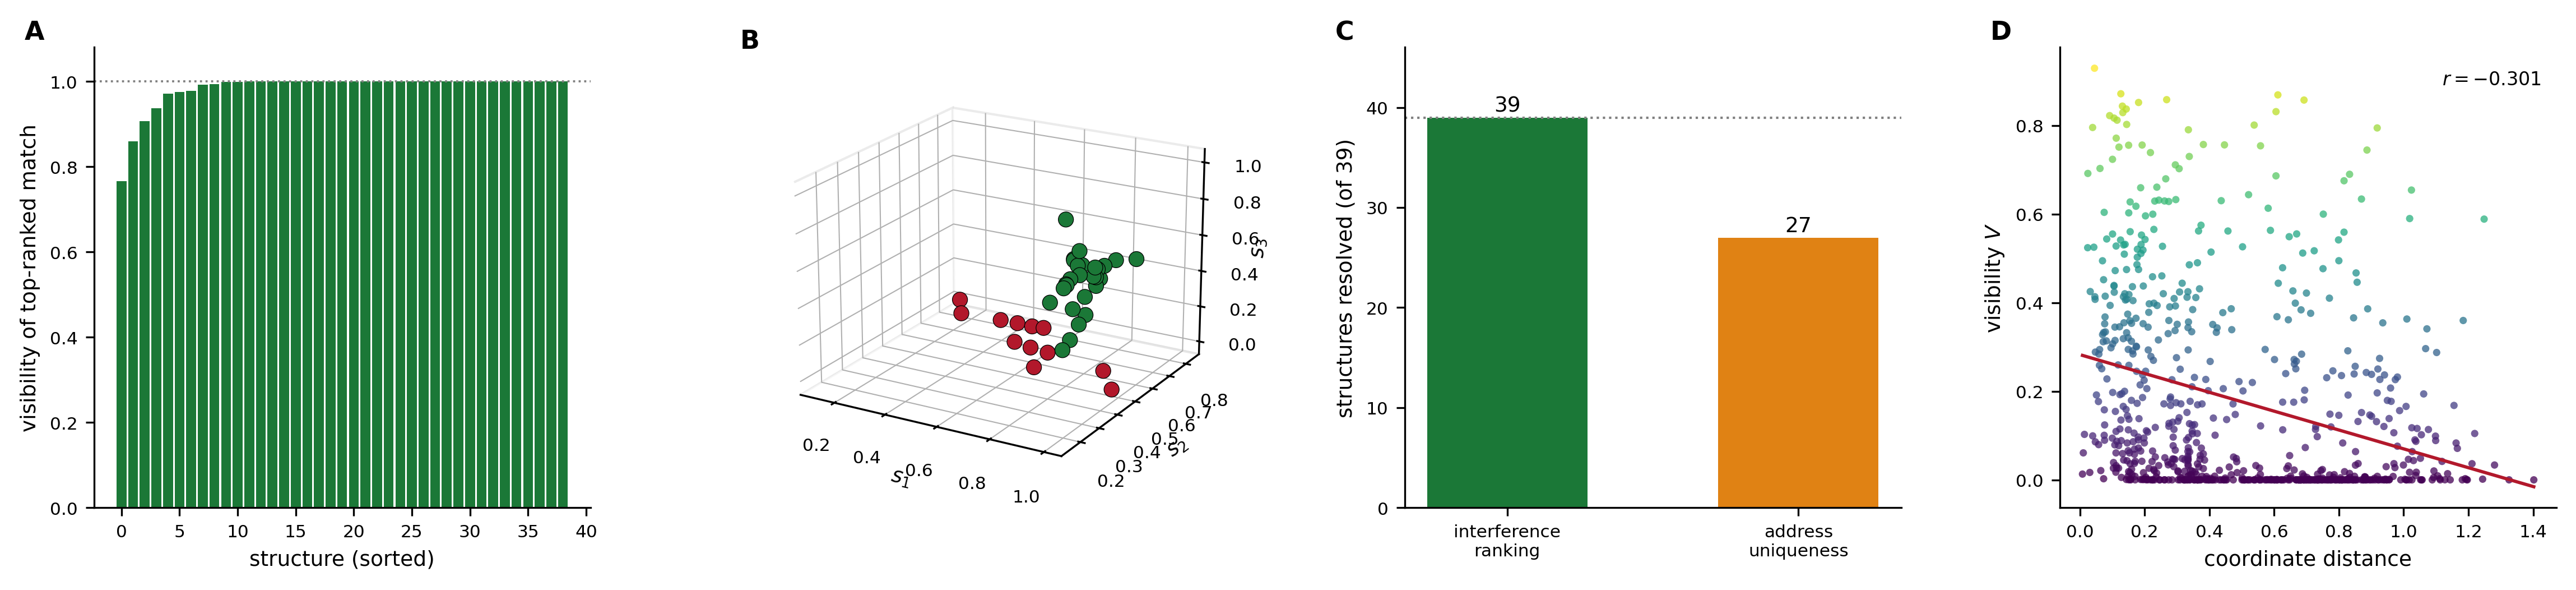
\includegraphics[width=\textwidth]{figures/panel_02_inversion.png}
    \caption{\textbf{Given a spectrum the instrument returns the
    structure that produced it, $39/39$ by interference; the addressing
    route resolves only $27/39$ and is a screen rather than an
    identification.}
    (\textbf{A})~Visibility of the top-ranked match for each of the $39$
    structures, sorted. The generating structure is ranked first in every
    case, and in all but a handful the top match sits at $V=1.0$ exactly
    --- the query field and the stored field coincide because the query
    is the same spectrum. The few bars below $1.0$ are structures whose
    stored record differs from the query in rounding only.
    (\textbf{B})~The $39$ structures at their coordinates
    $(s_1,s_2,s_3)$, coloured by whether the full-depth address names
    them uniquely: green resolved, red sharing a cell with at least one
    other structure. The twelve unresolved structures concentrate at low
    $s_3$, where the third coordinate --- the harmonic-ratio fraction ---
    takes few distinct values and therefore refines the address slowly.
    The failure is structured, not scattered.
    (\textbf{C})~The two routes side by side. Interference ranking
    resolves $39$ of $39$; address uniqueness resolves $27$, an accuracy
    of $0.692$. Reporting only the former would conceal that the
    addressing layer is a prefix screen with a $69.2\%$ unique-hit rate
    (\Cref{rem:routes}).
    (\textbf{D})~Visibility against coordinate distance for all $741$
    pairs, coloured by visibility, with a least-squares line. The
    correlation is $r=-0.301$: visibility falls with separation, as an
    interference measure must, but the relationship is loose. The large
    population at $V\approx0$ and moderate distance is the set of pairs
    whose modes simply do not overlap, for which the cross-term vanishes
    regardless of how far apart the coordinates are.}
    \label{fig:inversion}
\end{figure*}

\begin{figure*}[!htbp]
    \centering
    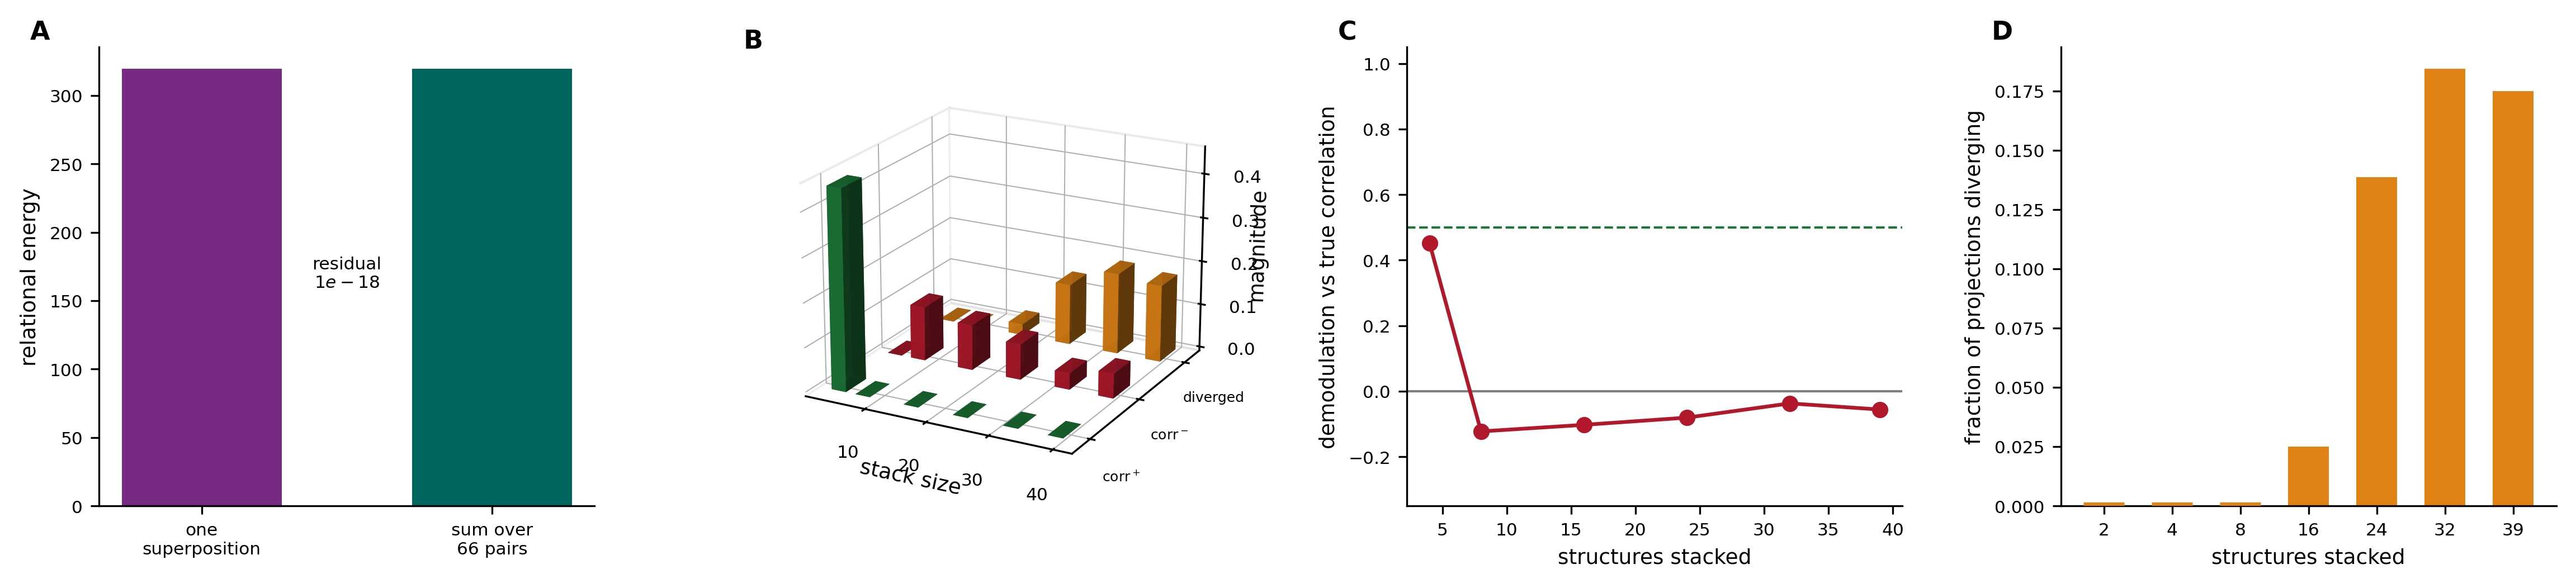
\includegraphics[width=\textwidth]{figures/panel_03_bulk.png}
    \caption{\textbf{The bulk identity holds exactly and buys nothing:
    a single superposition contains every pairwise cross-term, and no
    pair can be recovered from it.}
    This is the figure that refutes the scaling claim the construction
    appeared to support.
    (\textbf{A})~The relational energy of $12$ stacked structures
    obtained from one superposition, against the explicit sum over all
    $66$ pairs. The two agree at $319.357946$ with a relative residual of
    $0$: \Cref{thm:bulkid} is realised to double precision. Read alone,
    this panel says bulk comparison is free.
    (\textbf{B})~Demodulation outcome against stack size, decomposed into
    positive correlation (green), negative correlation (red) and the
    fraction of projections that diverge (orange). The green bar exists
    only at the smallest stack; from eight structures onward the
    correlation is negative and the orange fraction grows.
    (\textbf{C})~Correlation between the demodulated estimate and the
    true pairwise visibility, against stack size, with the $0.5$ level
    marked. It is $0.452$ at four structures, $-0.123$ at eight, and
    stays near zero thereafter. The $n=2$ point is omitted because a
    single pair provides no variance and its correlation is undefined
    rather than zero (\Cref{rem:n2}).
    (\textbf{D})~Fraction of projections diverging, per stack size, with
    genuine zeros drawn as floor ticks so they read as measured rather
    than absent. Divergence begins at $16$ structures ($2.5\%$) and
    reaches $17.5\%$ at $39$. The mechanism is \Cref{prop:nonorth}: the
    cross-term bases share support and are not orthogonal, so each
    projection absorbs energy belonging to other pairs. Panels
    (\textbf{A}) and (\textbf{C}) together are the paper's central
    finding --- the relational content is \emph{present} in the stack and
    \emph{not addressable} within it.}
    \label{fig:bulk}
\end{figure*}

\begin{figure*}[!htbp]
    \centering
    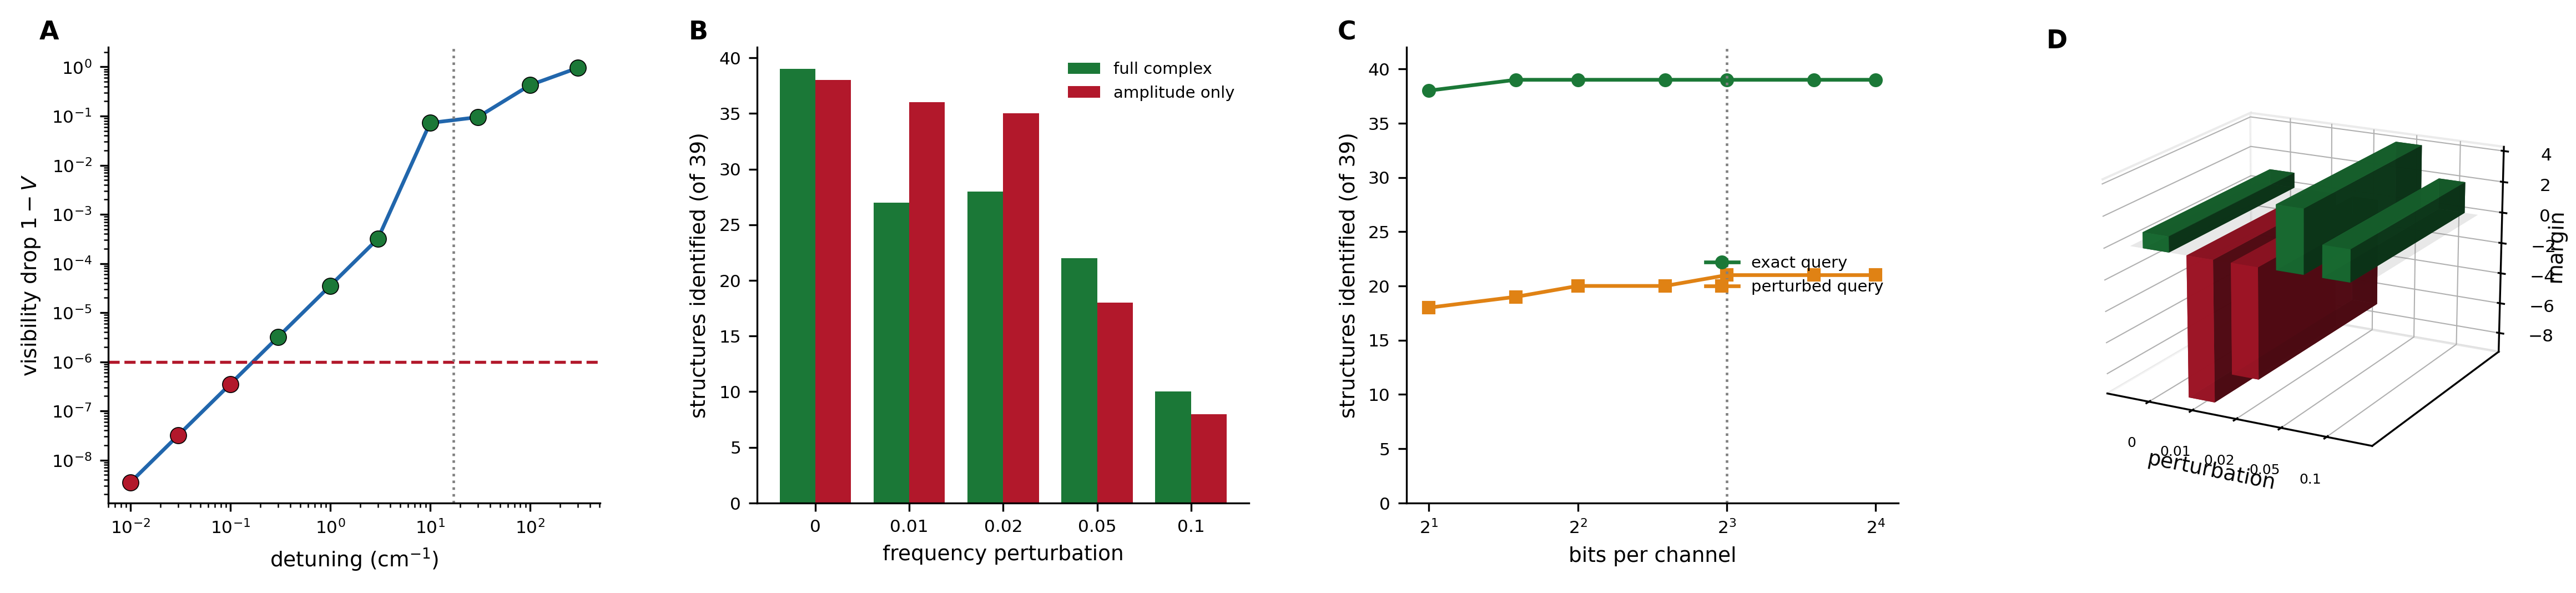
\includegraphics[width=\textwidth]{figures/panel_04_limits.png}
    \caption{\textbf{Three limits: the floor is declared rather than
    derived, the phase term is fragile, and display precision costs
    nothing.}
    (\textbf{A})~Visibility drop against detuning of one mode of a
    reference structure, on log--log axes, with the declared
    detectability threshold $10^{-6}$ (red dashed) and the grid cell
    width $17.19$~cm$^{-1}$ (grey dotted). Points are green where the
    drop exceeds the threshold and red where it does not. The smallest
    detectable detuning is $0.3$~cm$^{-1}$, a factor $0.017$ of the grid
    cell: the floor is not set by sampling, because the lobes are smooth
    and sampled rather than binned, so a sub-cell shift still moves every
    sample. What sets the floor is the threshold, which is an instrument
    parameter and must be declared (\Cref{rem:floorcriterion}).
    (\textbf{B})~The full complex comparison against an amplitude-only
    control, over increasing multiplicative frequency perturbation. The
    control \emph{beats} the full comparison at $1\%$ ($36$ against
    $27$) and $2\%$ ($35$ against $28$), and loses only from $5\%$
    onward. We had predicted the full comparison would dominate
    everywhere. The reading is that the accumulated phase of
    \Cref{eq:phase} is linear in mode frequency, so a small
    multiplicative perturbation of a high-frequency mode produces a large
    phase error and decoheres a comparison that amplitude alone would
    have got right.
    (\textbf{C})~Structures identified against bits per channel, for
    exact queries (green) and one fixed set of $5\%$ perturbed queries
    (orange), with $8$ bits marked. Both curves are flat from $8$ bits
    upward: $39/39$ and $21/39$ at $8$, $12$ and $16$ bits alike. Nothing
    measurable is lost by letting the displayed array be the compared
    array. An earlier version of this test drew fresh perturbations per
    depth and appeared to show low precision winning; that was a
    difference between query sets (\Cref{rem:rngartefact}).
    (\textbf{D})~The margin of panel~(\textbf{B}) --- full minus
    phaseless --- in three dimensions, with the zero plane drawn. Bars
    below the plane are perturbation levels at which the simpler control
    is better. The two red bars are the paper's clearest statement of
    where this construction should not be used: for spectra with
    sub-percent frequency uncertainty, an amplitude correlation is the
    better instrument.}
    \label{fig:limits}
\end{figure*}
